\section{Extra projects}

Some additional small projects were undertaken in parallel to ePATH Test Bench project.

\subsection{Electrical display switching}
To test the functionality of the device during animal studies, it was proposed that the Target and Crossing catheters are connected to three different ePATH displays. To make the change between displays as easy as possible without requiring the removal of the catheters from the animal's body a switching mechanism is required. While the mechanical switching between the displays with switches was already explored, an electrical decision was required. Some electrical components that would enable the switching were explored as follows.

\subsubsection{Background}
Firstly, the idea of using solid state relays(SSRs) was explored \cite{ssr_rfwireless}. A large advantage of using this is that SSRs are optically isolated. Therefore, the input and output are physically isolated when the current is below a certain level which enhances precision by minimizing noise. This will be very useful in this system as interferences from the different displays will have no effect on how the system behaves. Other advantages include their ability to work with both DC and AC signals, their silent operation and low power consumption. A problem when working with SSRs is that they break easily. 

Secondly, transistors were considered as an alternative switching method as they are widely used as switches \cite{transistor_switch}.  They offer a wide range of advantages such as current control, controlling the exact current that would enter the ePATH display, and offer quick switching. Transistors can be arranged in Darlington or Sziklai configurations which increases the input impedance further. There is a wide variety of transistors for different operating conditions thus choosing the appropriate transistor involves more calculations. A big disadvantage is that the inputs and outputs are not isolated so even if the transistor if off there might be some leakage current that interferes with the operation of the system.

Multiplexers can also function as switches. For example, the SN74CBT16214CDLR \cite{sn74cbt_datasheet} provides twelve independent 3:1 MUX channels that could be used for this purpose. However, once again there is a direct physical connection between the inputs and outputs. This could pose problems if the circuit is not powered or if the MUX malfunctions, potentially allowing unintended signal paths. Controlling the MUX with an Arduino would also increase the system’s complexity. Furthermore, there are limitations on which ports can be used simultaneously, which could restrict potential future expansions of the project.

Tri-state buffers were also considered to be used as switches. They enable or disable the connection between input and output via changes in impedance \cite{digital_buffer}. However, they were quickly ruled out upon determining that their output is limited to only three states: logic high (1), logic low (0), or high impedance (Z). As a result, they cannot transmit complex analogue signals, which are the type of signals involved in our application. Another component that was quickly rejected was the silicon-controlled rectifier (SCR) \cite{scr_switch}. The main drawback is the difficulty of turning off a conducting SCR, which requires specialized commutation circuits to force the switch open. Additionally, SCRs can unintentionally turn on due to a high rate of voltage change (dv/dt) at the source which might occur due to electrical interference. It should be noted however that one advantage of the SCR, compared to a transistor, is that it operates strictly in binary states: either fully on or fully off, with no active region of operation.

For the reasons outlined above, particularly the significant advantage of opto-isolation, relays were selected to implement the electrical switches. These relays will be controlled by shift registers, which are themselves managed by an Arduino. Shift registers were chosen as they are relatively easy to control and have flexible functionality allowing many pins to be on simultaneously.

\subsubsection{Design proposition}
Design one:

The crossing catheter has 4 connecting wires and the target catheter 2. Therefore, 6 connections per display need to be switched on and off. Since there are 3 displays, this is an overall of 18 connections that need to be controlled. Therefore, 18 Single Pole Single Throw(SPST) relays would need to be used, or 9 Single Pole Double Throw relays like ASSR-1420-302E \cite{assr_datasheet} or 6 Single Pole Thee Throw relays like FMSW6362 \cite{relay_switch. These can be controlled by 8-bit shift registers like SN74AHCT595PWR \cite{shift_register}. The block diagram below shows the connection between a particular pin on a catheter and it’s corresponding connecting point with the displays when using SPST relays. Another 15 such connections would need to be wired.

\begin{figure}[H]
          \centering
          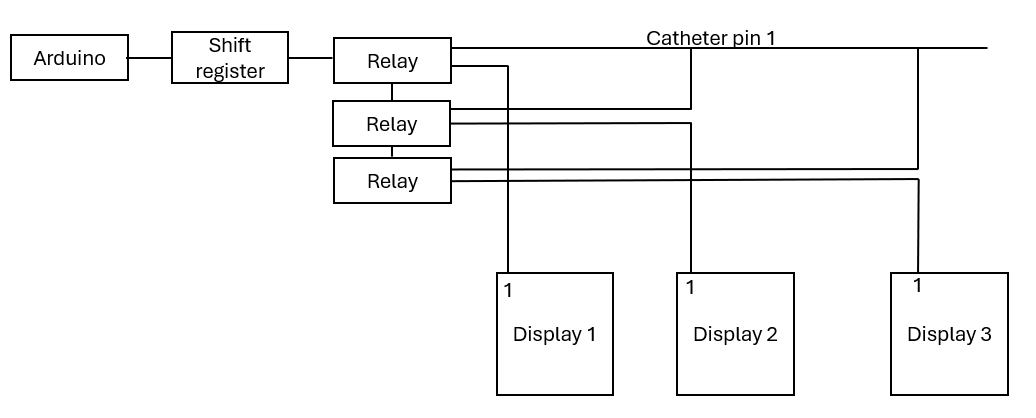
\includegraphics[width=1\linewidth]{img/Design1.png}
          \caption{Block diagram of first design proposition}
          \label{button_wiring}
    \end{figure}
    
A disadvantage of this design is the large amount of relays and thus wiring needed.

Design two:

In order to minimize the number of relays and connections needed, an alternative solution is to connect the inputs of the 3 displays and selectively turn on the display we want to use. This would mean that data is sent to all displays but only the display that is turned on is processing it.
To turn on and off the appropriate display, relays can be used. Each display is powered by 2 wires; the ground and the voltage wire. The ground connection of all the displays can be connected. The voltage wire of each display can be switched on and off using 3 SPST relays controlled by a shift register.  The block diagram of such a connection is shown below.
\begin{figure}[H]
          \centering
          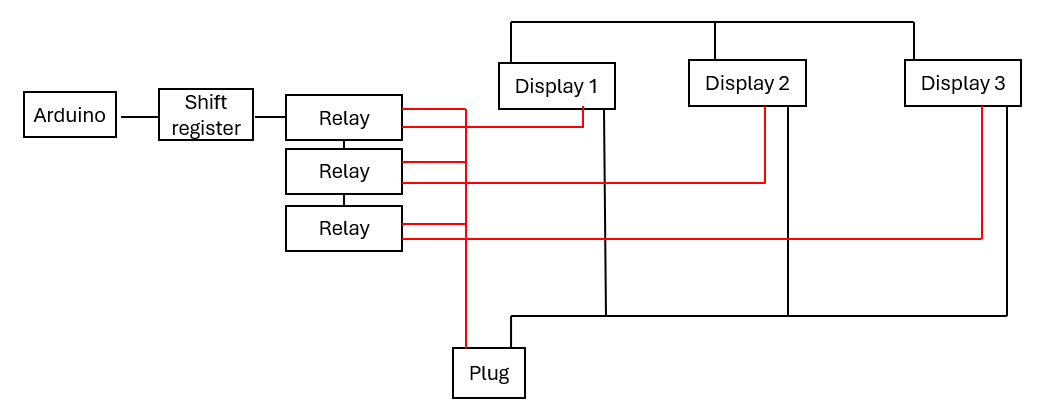
\includegraphics[width=1\linewidth]{img/Design2.png}
          \caption{Block diagram of second design proposition}
          \label{button_wiring}
    \end{figure}
An issue with this wiring method is that when sending commands to a display that is turned off some interference can be created which will affect its functionality when it’s turned on. Another issue is that the displays take some time to turn on thus this method would be slower. Therefore, this is deemed a worse design than Design 1.


\subsubsection{Conclusion}
In conclusion, to electrically switch the catheter connections between the three ePATH displays, a combination of relays and shift registers was determined to be the most effective solution. Among the configurations considered, Design 1 was found to be the most suitable for implementing the system with minimal interference.





\subsection{Text file saving}
Data printed in the Serial monitor of Arduino IDE can easily be lost and is difficult to work with. To make data acquisition and handling easier, a simple GUI was developed that captures the printed data and saves it in a .txt file. The GUI consists of a:
\begin{itemize}
\item A list-box that displays the information printed on the Serial monitor. 
\item A save button that saves the data in a text file at the desired directory.
\item A clear button that deletes data in case they were corrupted.
\item A information button that displays an information window that explains the GUI's functionalities.
\end{itemize}

The python code used to develop this GUI is in the resources folder of this document under the name Save text files. An Arduino code that prints out the numbers from 1-100 is also provided for demonstrative purposes.

\begin{table*}[ht]
    \centering
    \begin{tabular}{p{0.25\linewidth}p{0.25\linewidth}p{0.25\linewidth}}
    \hline
    column 1 & column 2 & column 3\\
    \hline
    1 & 2 & 3\\
    1 & 2 & 3\\
    1 & 2 & 3\\
    1 & 2 & 3\\
    \hline
    \end{tabular}
    \caption{Another random table}
    \label{tab:2}
\end{table*}
\noindent Another type of table for your results below.

\subsection{Subtopic 2}
\lipsum[1]

\noindent Another figure grid example: (on next page)

\begin{figure*}[ht]
\begin{multicols}{2}
        \centering
        \begin{subfigure}[b]{0.475\textwidth}
            \centering
            
\includegraphics[width=\textwidth]{img/bioeng.jpg}
            \caption{Part 1}    
        \end{subfigure}
        \hfill
        \begin{subfigure}[b]{0.475\textwidth}  
            \centering 
            
\includegraphics[width=\textwidth]{img/bioeng.jpg}
            \caption{Part 2}    
        \end{subfigure}
        \vskip\baselineskip
        \begin{subfigure}[b]{0.475\textwidth}   
            \centering 
            
\includegraphics[width=\textwidth]{img/bioeng.jpg}
            \caption{Part 3}  
        \end{subfigure}
        \hfill
        \begin{subfigure}[b]{0.475\textwidth}   
            \centering 
            
\includegraphics[width=\textwidth]{img/bioeng.jpg}
            \caption{Part 4}    
        \end{subfigure}
        \label{fig:mean and std of nets}
        \end{multicols}
        \caption {A figure grid} 
        \label{fig:3}
    \end{figure*}
